% !TEX TS-program = pdflatex
% !TEX encoding = UTF-8 Unicode

% This file is a template using the "beamer" package to create slides for a talk or presentation
% - Talk at a conference/colloquium.
% - Talk length is about 20min.
% - Style is ornate.

% MODIFIED by Jonathan Kew, 2008-07-06
% The header comments and encoding in this file were modified for inclusion with TeXworks.
% The content is otherwise unchanged from the original distributed with the beamer package.

\documentclass{beamer}


% Copyright 2004 by Till Tantau <tantau@users.sourceforge.net>.
%
% In principle, this file can be redistributed and/or modified under
% the terms of the GNU Public License, version 2.
%
% However, this file is supposed to be a template to be modified
% for your own needs. For this reason, if you use this file as a
% template and not specifically distribute it as part of a another
% package/program, I grant the extra permission to freely copy and
% modify this file as you see fit and even to delete this copyright
% notice. 


\mode<presentation>
{
  \usetheme{Warsaw}
  % or ...

  \setbeamercovered{transparent}
  % or whatever (possibly just delete it)
}
\setbeamertemplate{navigation symbols}{}

\usepackage[english]{babel}
% or whatever

\usepackage[utf8]{inputenc}
% or whatever

\usepackage{times}
\usepackage[T1]{fontenc}
% Or whatever. Note that the encoding and the font should match. If T1
% does not look nice, try deleting the line with the fontenc.


\title[Monitoring BitTorrent swarms \hspace{26mm} \insertframenumber/\inserttotalframenumber] % (optional, use only with long paper titles)
{Monitoring BitTorrent swarms}

\subtitle
{}

\author[António Homem Ferreira] % (optional, use only with lots of authors)
{António Homem Ferreira \\ Student nº 55935 \\ MERC}
% - Give the names in the same order as the appear in the paper.
% - Use the \inst{?} command only if the authors have different
%   affiliation.

\institute[Universities of Somewhere and Elsewhere] % (optional, but mostly needed)
{
  INESC-ID, Communications Networks and Mobility\\
  Instituto Superior Técnico - Campus TagusPark
}
% - Use the \inst command only if there are several affiliations.
% - Keep it simple, no one is interested in your street address.

\date[CFP 2003] % (optional, should be abbreviation of conference name)
{}
% - Either use conference name or its abbreviation.
% - Not really informative to the audience, more for people (including
%   yourself) who are reading the slides online

\subject{Theoretical Computer Science}
% This is only inserted into the PDF information catalog. Can be left
% out. 



% If you have a file called "university-logo-filename.xxx", where xxx
% is a graphic format that can be processed by latex or pdflatex,
% resp., then you can add a logo as follows:

\pgfdeclareimage[height=0.5cm]{university-logo}{figures/logo_ist}
\logo{\pgfuseimage{university-logo}}



% Delete this, if you do not want the table of contents to pop up at
% the beginning of each subsection:



% If you wish to uncover everything in a step-wise fashion, uncomment
% the following command: 

%\beamerdefaultoverlayspecification{<+->}


\begin{document}

\begin{frame}
  \titlepage
\end{frame}

\begin{frame}{Outline}
  \tableofcontents[section]
\end{frame}


% Structuring a talk is a difficult task and the following structure
% may not be suitable. Here are some rules that apply for this
% solution: 

% - Exactly two or three sections (other than the summary).
% - At *most* three subsections per section.
% - Talk about 30s to 2min per frame. So there should be between about
%   15 and 30 frames, all told.

% - A conference audience is likely to know very little of what you
%   are going to talk about. So *simplify*!
% - In a 20min talk, getting the main ideas across is hard
%   enough. Leave out details, even if it means being less precise than
%   you think necessary.
% - If you omit details that are vital to the proof/implementation,
%   just say so once. Everybody will be happy with that.

\section{Motivation}

\begin{frame}{Motivation}

 Increasing usage of P2P communications
\\
 BitTorrent accounts for 60\% of worldwide P2P traffic

\begin{figure} [h]
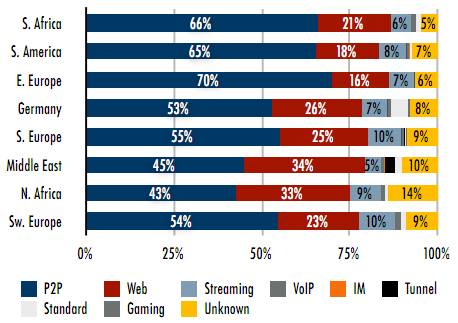
\includegraphics[height=1.85in]{figures/PercentagemP2P_total}
\caption{Ipoque's Internet Study 2008/2009}
\label{fig:1} 
\end{figure}

\end{frame}


\begin{frame}{Motivation}

\begin{itemize}
\addtolength{\itemsep}{1.5\baselineskip}
\item
   P2P protocols generate a great amount of traffic
\item
   Affects quality of service of other protocols

\item
   P2P communications results in high inter-ISP traffic 
\item
   Inter-ISP traffic is expensive for ISPs

\end{itemize}

\end{frame}



\section{Work Objectives}

\begin{frame}{Work Objectives}

\begin{itemize}
\addtolength{\itemsep}{1.2\baselineskip}
\item
   Study monitoring real Internet BitTorrent swarms 
\item
   Data gathered used to identify patterns in BitTorrent networks:

\begin{itemize}
\item
   Locality - decrease inter-ISP traffic
\item
   Content - increase content availability

\end{itemize}
\end{itemize}

\end{frame}


\section{The BitTorrent Protocol}

\begin{frame}{BitTorrent Protocol}

File-sharing protocol

\begin{itemize}
\item
   Peers share files among themselves
\item
   Files are divided into smaller pieces
\item
   Central Server (Tracker) which provides a list of active peers
\item
   Mechanisms that make peers chose to download from the ones with the largest bandwidth
\end{itemize}

\end{frame}



\section{Contributions}

\begin{frame}{Contributions}
This study differs in:
\begin{itemize}
\addtolength{\itemsep}{1\baselineskip}
\item
    Locality studied for two different periods
\item
   Content study that focuses on repeated content
\item
   PSM - an approach to increasing content availability 
\item
   Peer and Tracker behaviors that can affect locality
\end{itemize}
\end{frame}


\section{Work Methodology}

\begin{frame}{Methodology for gathering data}

\begin{figure}
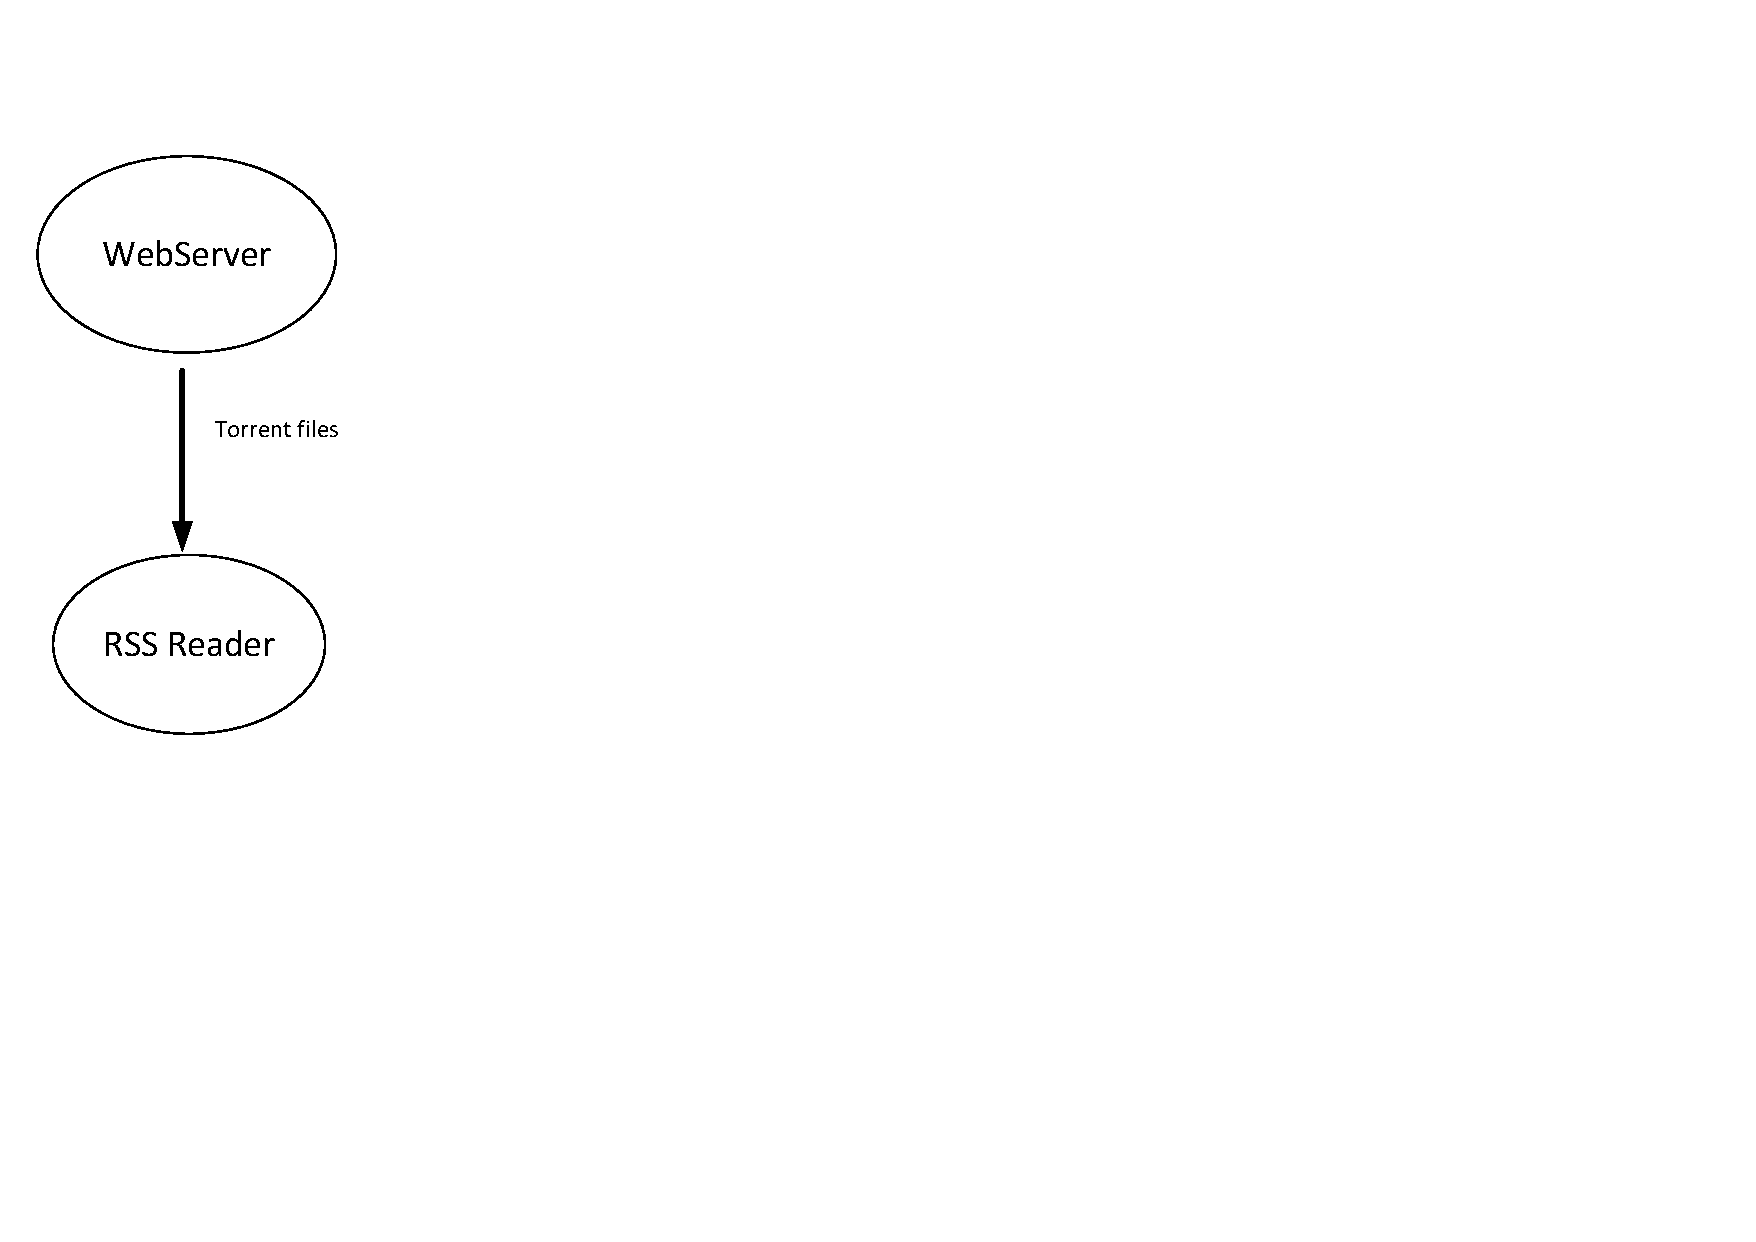
\includegraphics[height=2.5in]{figures/ArqSimplesV2_1}
\label{fig:3} 
\end{figure}

\end{frame}

\begin{frame}{Methodology for gathering data}

\begin{figure}
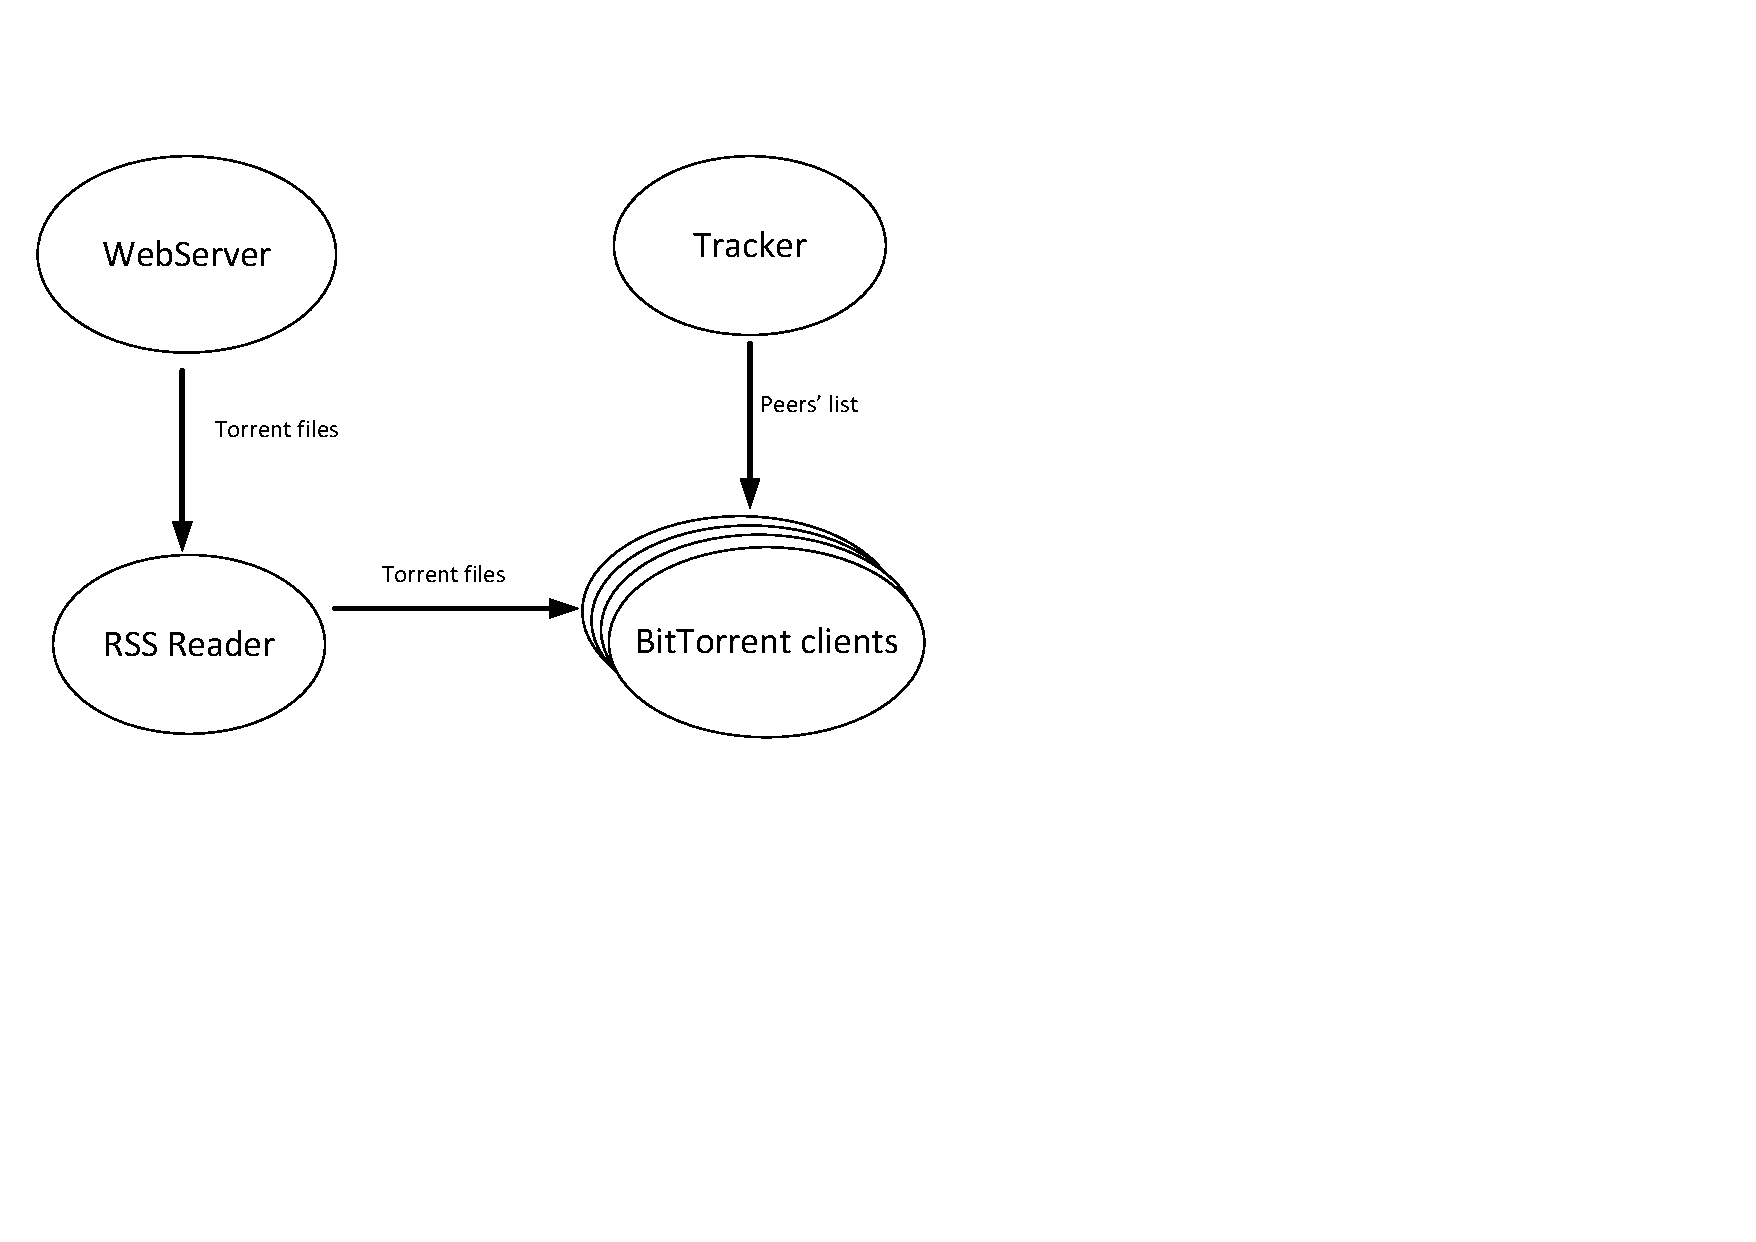
\includegraphics[height=2.5in]{figures/ArqSimplesV2_2}
\label{fig:4} 
\end{figure}

\end{frame}

\begin{frame}{Methodology for gathering data}

\begin{figure}
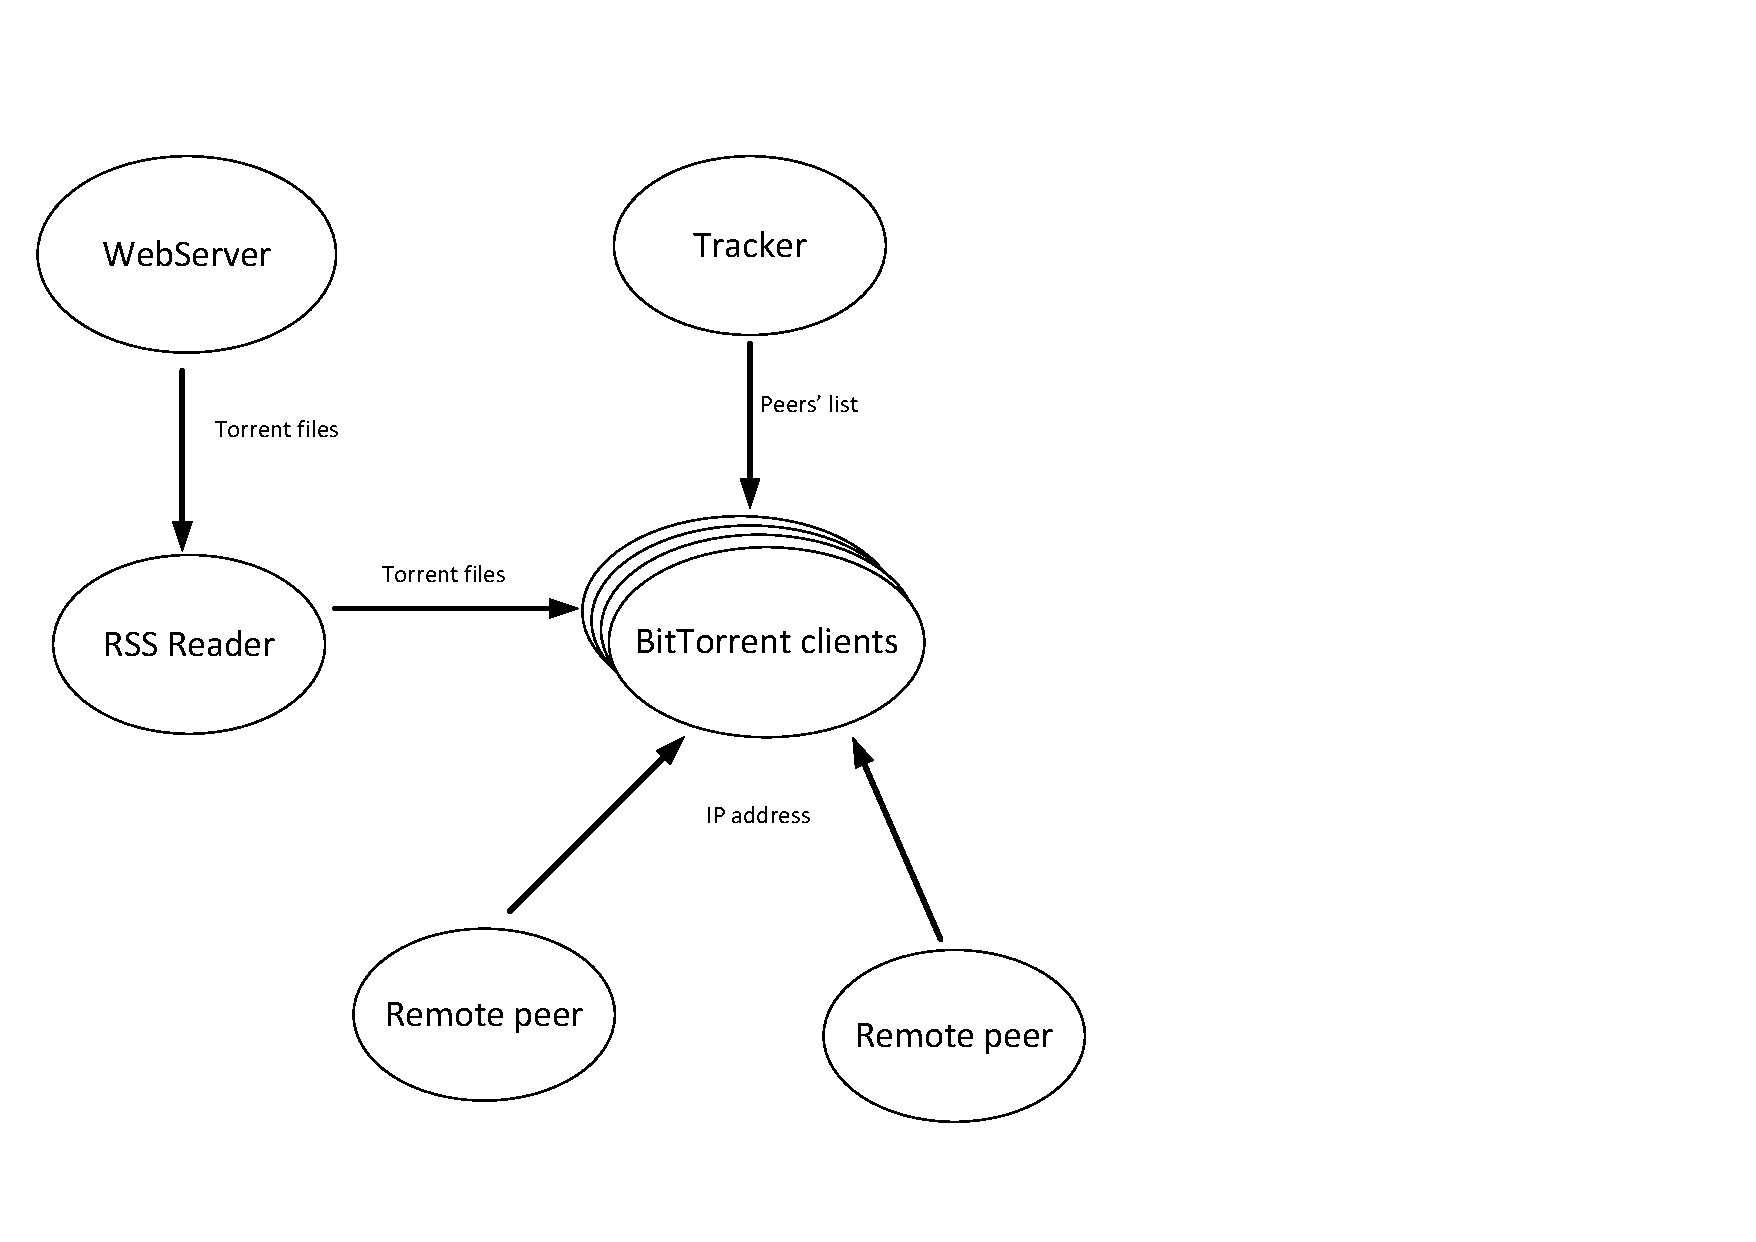
\includegraphics[height=2.5in]{figures/ArqSimplesV2_3}
\label{fig:5} 
\end{figure}

\end{frame}

\begin{frame}{Methodology for gathering data}

\begin{figure}
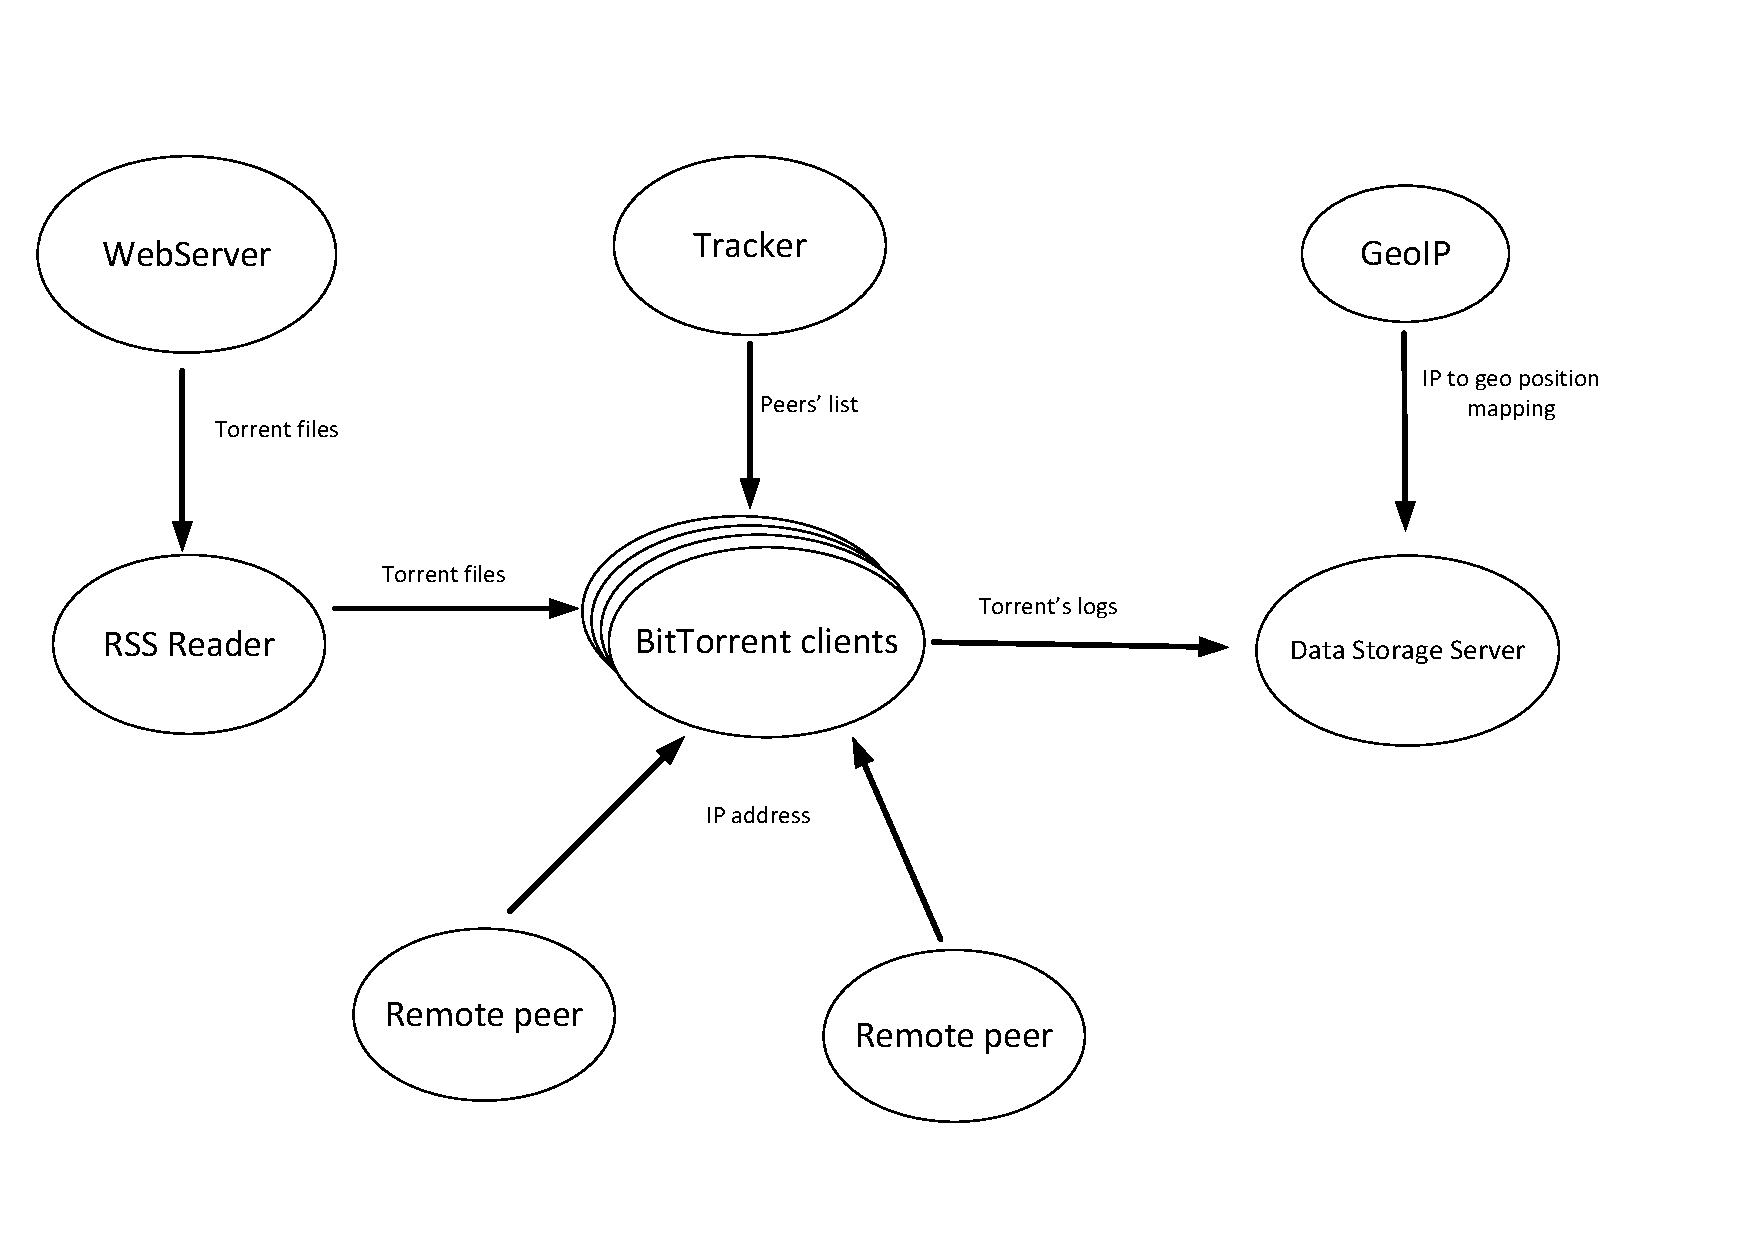
\includegraphics[height=2.5in]{figures/ArqSimplesV2}
\label{fig:6} 
\end{figure}

\end{frame}



\begin{frame}{Methodology for analyzing data}

The torrent database:
\begin{itemize}
\addtolength{\itemsep}{1\baselineskip}
\item
   3211 torrent files from PirateBay, isohunt and btjunkie
\item
   Torrent files collected from the 25$^{th}$ of April 2011 to the 18$^{th}$ of July 2011
\item
   PirateBay's one hundred most popular torrent files on the 25$^{th}$ of April
\item
   isohunt's twenty most popular torrent files on the 24$^{th}$ of May for each major category (audio, video, and tv)
\end{itemize}
\end{frame}

\begin{frame}{Methodology for analyzing data}

\begin{itemize}
\addtolength{\itemsep}{1\baselineskip}
\item Different data analysis criteria for each study:
\begin{itemize}
\item
   Locality study
\item
   Content study
\end{itemize}

\item
   Monitoring stopped for all swarms that dropped below 30 peers and 0 seeders for a period of a week

\item
  Monitoring nodes not part of the results.
\end{itemize}
\end{frame}



\section{Results}

\begin{frame}{Results}

\begin{itemize}
\addtolength{\itemsep}{1\baselineskip}
\item
    Locality Analysis
\item
     Content Analysis
\item
     Peer and tracker behavior
\end{itemize}
\end{frame}


\begin{frame}{Locality Analysis}

\begin{figure}[h]
\center
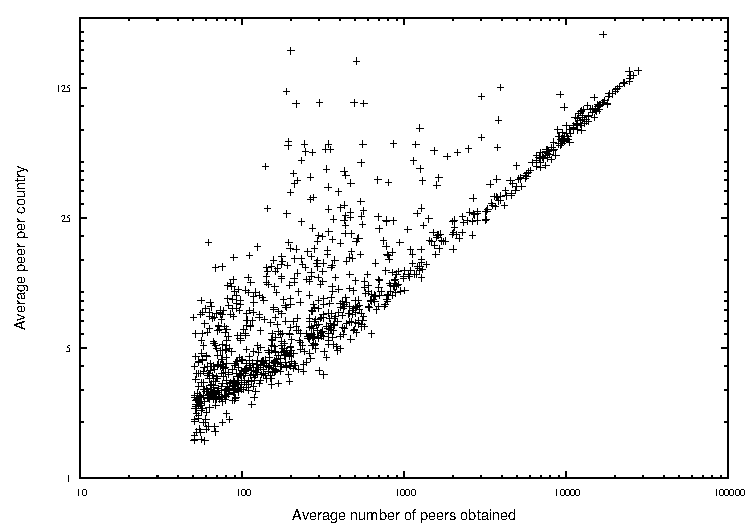
\includegraphics[height=1.85in]{Figures/countryPeers_AVGPerPeers}
\caption{Average number of peers obtained and average number of peers per country.}
\label{fig:torrent_avg_country} 
\end{figure}

\end{frame}


\begin{frame}{Locality Analysis}

\begin{figure}[h]
\center
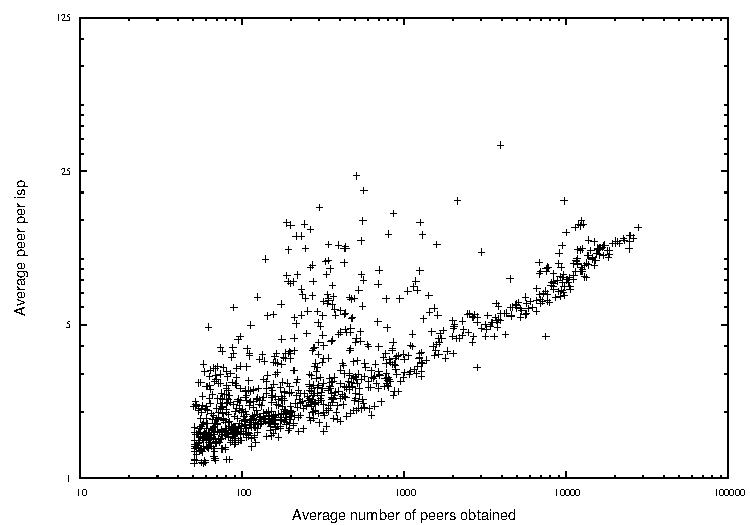
\includegraphics[height=1.85in]{Figures/ispPeers_AVGPerPeers}
\caption{Average number of peers obtained and average number of peers per ISP.}
\label{fig:torrent_avg_isp} 
\end{figure}

\end{frame}



\begin{frame}{Locality Analysis - Regional content}

\begin{figure}[h]
\center
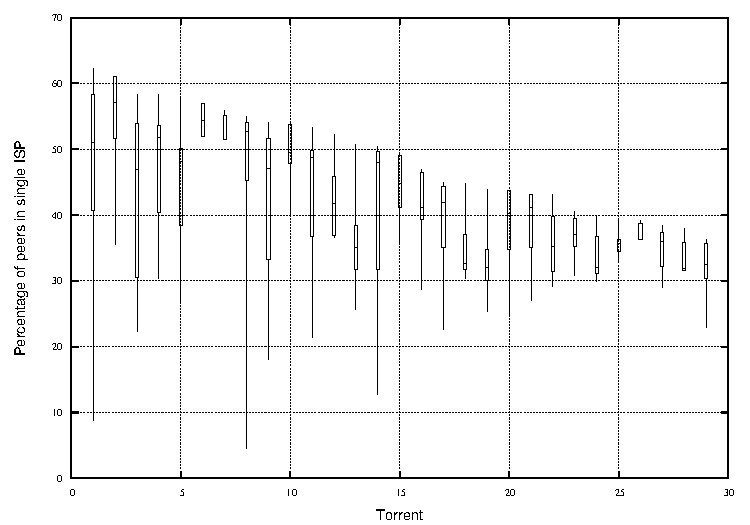
\includegraphics[height=1.85in]{Figures/ispPeers_candlestick_above30}
\caption{Regional torrents with 30\% of all peers belonging to the same ISP, at least 75\% of the times.}
\label{fig:torrent_avg_isp} 
\end{figure}

\end{frame}


\begin{frame}{Content Analysis}

\begin{itemize}
\addtolength{\itemsep}{1\baselineskip}
\item
    Content pollution
\item
    Content repetition

\end{itemize}
\end{frame}


\begin{frame}{Content Analysis - Content pollution}

\begin{itemize}
\addtolength{\itemsep}{1\baselineskip}
\item
    Files with most parts the same
\item
    Files did not represent any real content
\item
   From the 3211 files collected, 221 were found to be polluted content

\end{itemize}

\end{frame}


\begin{frame}{Content Analysis - Content repetition}

\begin{figure}[h]
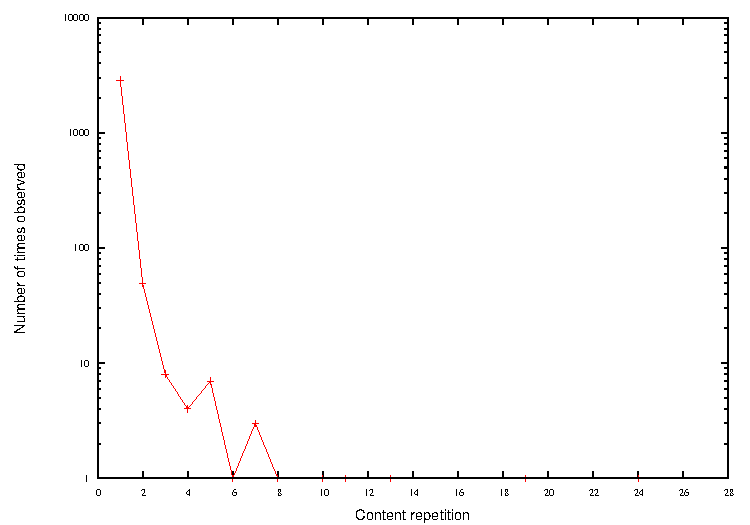
\includegraphics[height=1.85in]{figures/NumContentPerSome}
\caption{Histogram of the content repetition frequency.}
\label{ctrep:2} 
\end{figure}

\end{frame}


\begin{frame}{Content Analysis - Content repetition}

\begin{figure}[h]
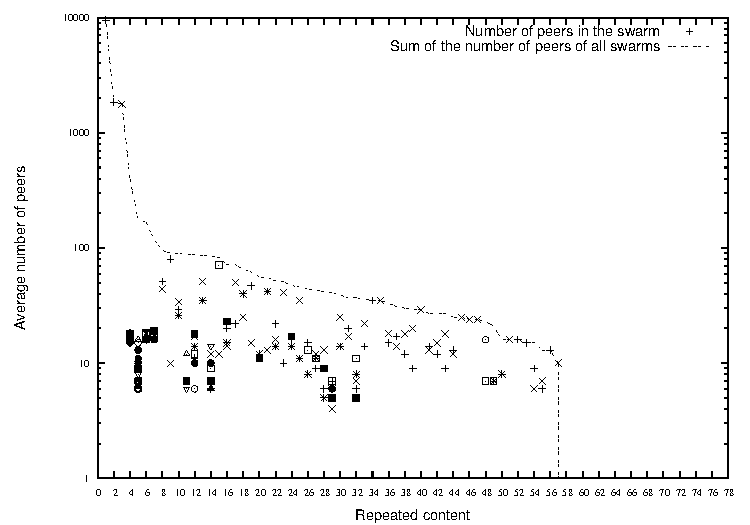
\includegraphics[height=1.85in]{figures/PeersPerContent}
\caption{Average number of peers per content.}
\label{ctrep:3} 
\end{figure}

\end{frame}

\begin{frame}{Content Analysis - Content repetition}

\begin{table}
\renewcommand{\arraystretch}{1.1}
\label{table:aggregation_benefits}
\begin{center}
\begin{tabular}{l||r|r|r|r}
\hline
 & Torrent 1 & Torrent 2 & Torrent 3 & Total \\
\hline \hline
Num. Countries & 87 & 68 & 38 & 101 \\
Avg. Peers/Country & 6.20 & 5.25 & 2.61 & 9.85 \\
Num. ISPs & 238 & 178 & 54 & 342 \\
Avg. Peers/ISP & 2.26 & 2.01 & 1.83 & 2.91 \\
\hline
\end{tabular}
\end{center}
\caption{Torrent aggregation benefits.}
\end{table}

\end{frame}

\section{Partial Swarm Merger}

\begin{frame}{PSM}

\begin{itemize}
\addtolength{\itemsep}{1\baselineskip}
\item
    Peers query for swarms that share similar content to the one they are currently downloading
\item
   Peers participate in multiple swarms, isolated from each other
\item
   Its databases are populated through the different queries received
\end{itemize}
\end{frame}


\begin{frame}{PSM}

\begin{itemize}
\addtolength{\itemsep}{1\baselineskip}
\item
    Service outside BitTorrent
\item
    Requires no modifications to the BitTorrent protocol
\item
   BitTorrent client application requires only an extension/add-on to make use of the service
\end{itemize}

\end{frame}


\begin{frame}{PSM}

\begin{figure}[h]
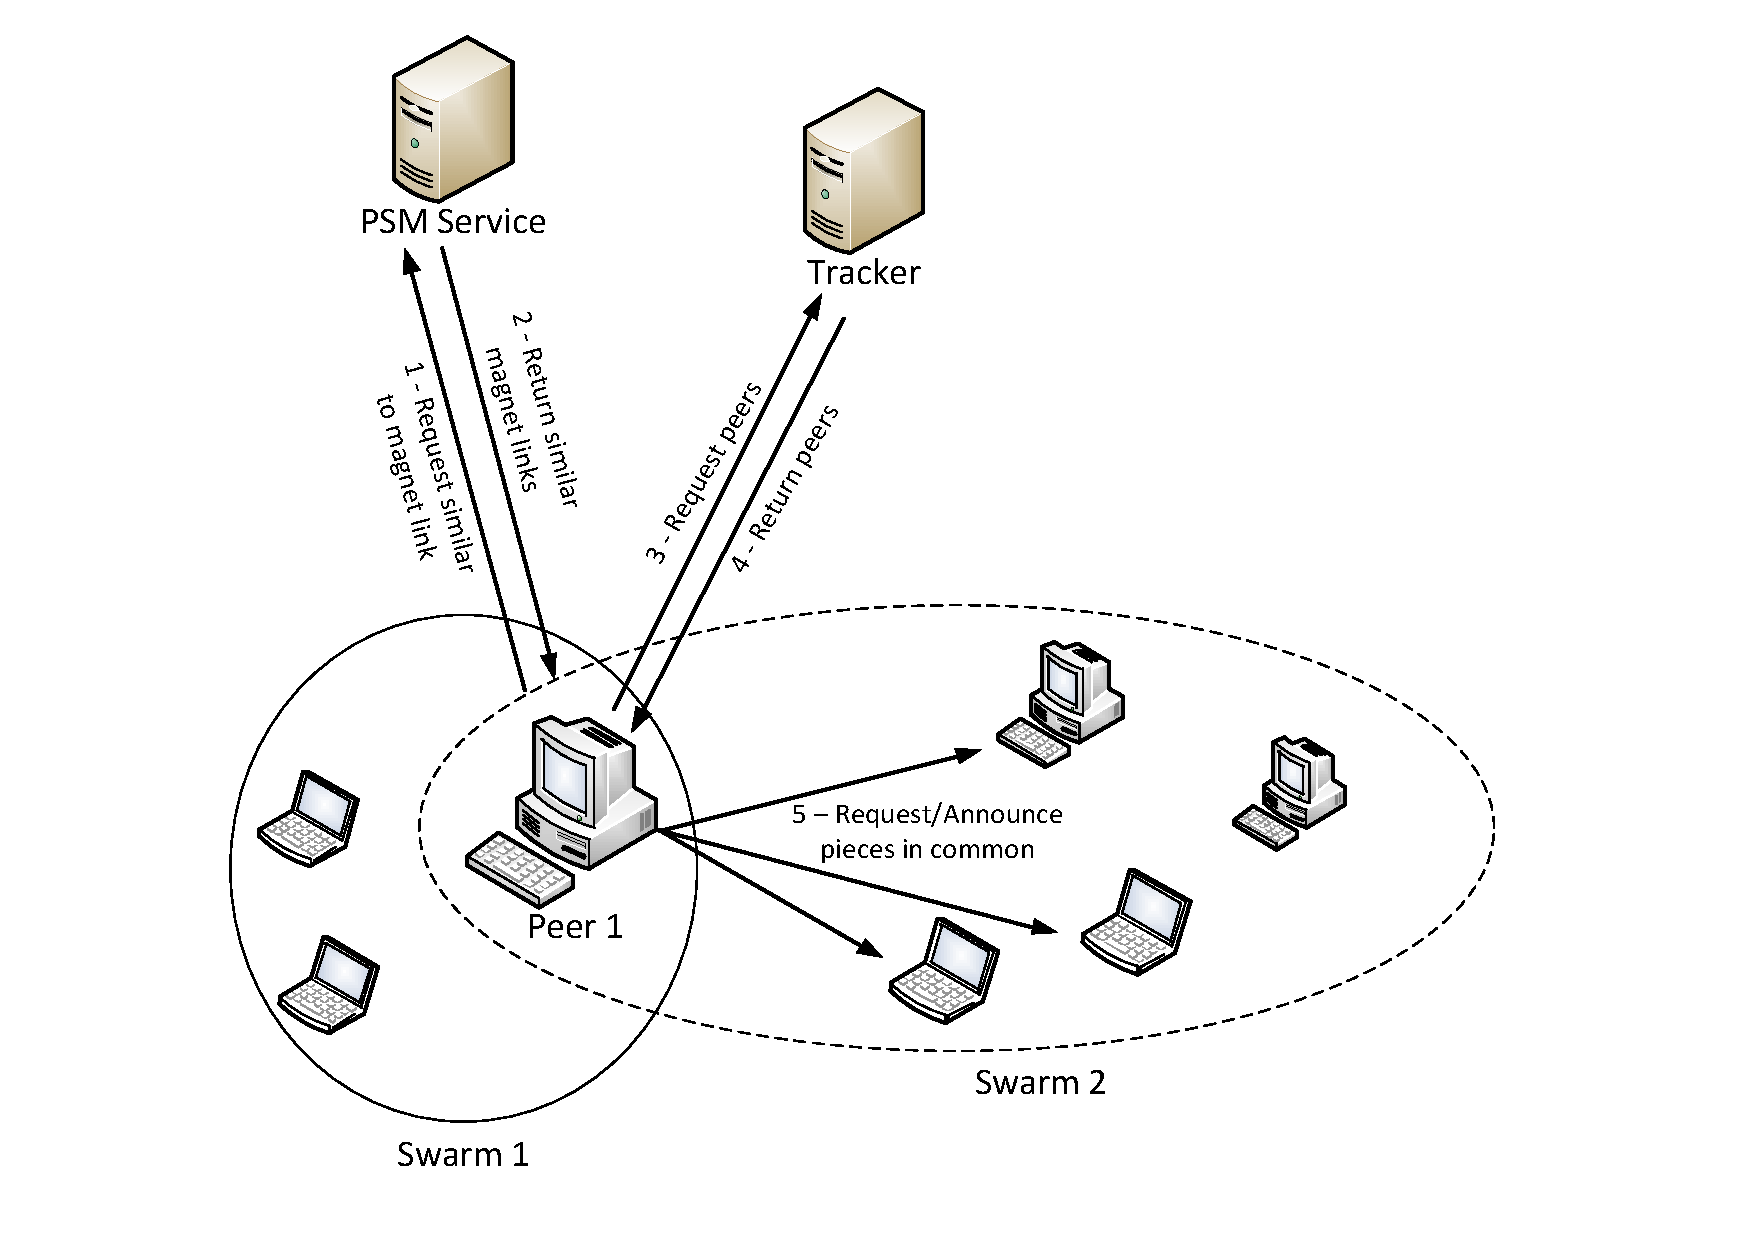
\includegraphics[height=1.85in]{figures/PSM-Workflow2}
\caption{PSM workflow.}
\label{ctrep:2} 
\end{figure}

\end{frame}

\section{Conclusions}

\begin{frame}{Conclusions}

\begin{itemize}

\addtolength{\itemsep}{1\baselineskip}
\item
    High locality properties in both large and small size swarms
\item
    Many patterns observed:
\begin{itemize}
\addtolength{\itemsep}{1\baselineskip}
\item
   Content shared
\item
   Peer behavior
\end{itemize}

\item
   Findings suggest that BitTorrent traffic can be restrained and inter-ISP traffic decreased

\end{itemize}

\end{frame}

\subsection*{}

\begin{frame}{Publications}
  
This paper was submitted to be presented at INFOCOM'2012 and we are now waiting for its evaluation.
\begin{list}{*}{}
\item António Homem Ferreira, Ricardo Lopes Pereira and Fernando M. Silva. Partial Swarm Merger: Increasing BitTorrent content availability.
\end{list}

\end{frame}


\end{document}


